\documentclass[12pt,a4paper]{article}

\usepackage[utf8]{inputenc}
\usepackage[T1]{fontenc}
\usepackage[brazil]{babel}
\usepackage{lmodern}
\usepackage{geometry}
\usepackage{graphicx}
\usepackage{amsmath}
\usepackage{amssymb}
\usepackage{booktabs}
\usepackage{array}
\usepackage{multirow}
\usepackage{xcolor}
\usepackage{hyperref}
\usepackage{float}
\usepackage{caption}
\usepackage{subcaption}
\usepackage{enumitem}

\geometry{margin=2.5cm}
\hypersetup{
    colorlinks=true,
    linkcolor=blue!50!black,
    citecolor=blue!50!black,
    urlcolor=blue!50!black
}

\graphicspath{
    {figures/}
    {paper/figures/}
}

\title{
    \textbf{ACDLR: um metodo classico e explicavel para deteccao de crateras lunares}\\
    \large Comparacao com Ellipse R-CNN e estudo qualitativo de objetos circulares em outros dominios
}

\author{
    \begin{tabular}{c}
        Marcos Henrique\\
        Diogo Nascimento\\
        Rafael de Souza\\[0.4em]
        \small Projeto de Visao Computacional
    \end{tabular}
}

\date{2026}

\begin{document}

\maketitle

\begin{abstract}
Este artigo apresenta o ACDLR (\textit{Automated Crater Detection and Landing Risk}), um sistema de visao computacional classica para deteccao de crateras lunares em imagens visuais e estimativa de risco visual de pouso por regiao. O metodo principal nao utiliza redes neurais, aprendizado profundo ou treinamento supervisionado. Em vez disso, combina pre-processamento por realce de contraste, deteccao de bordas, filtragem circular multi-escala, validacao geometrica e fotometrica, refinamento local e deduplicacao. A avaliacao principal e realizada em um dataset visual anotado no formato YOLO, com conversao das anotacoes para circulos. Como baseline neural externo, utiliza-se Ellipse R-CNN com pesos pre-treinados para crateras, especificamente o modelo \texttt{wdoppenberg/crater-rcnn}. Alem da avaliacao lunar, o artigo discute uma extensao qualitativa para imagens de objetos circulares com contraste forte em relacao ao fundo, incluindo um exemplo de imagens celulares com bom comportamento e um estudo de buracos em ruas com desempenho mais limitado devido a poluicao visual, variacao de iluminacao e baixa circularidade. Os resultados obtidos indicam que o ACDLR apresenta desempenho competitivo no teste oficial de crateras, com interpretabilidade superior e sem custo de treinamento local, embora sua generalizacao para dominios nao lunares dependa fortemente da estrutura visual dos objetos.
\end{abstract}

\textbf{Palavras-chave:} deteccao de crateras; visao computacional classica; CLAHE; filtros circulares; objetos circulares; Ellipse R-CNN; analise de risco visual.

\section{Introducao}

A deteccao de crateras lunares e um problema classico em visao computacional aplicada a ciencias planetarias, navegacao autonoma e analise de terreno. Crateras sao estruturas morfologicas abundantes na Lua e podem servir como referencias visuais para localizacao, mapeamento, interpretacao geologica e avaliacao de regioes de pouso. Entretanto, sua deteccao automatica e desafiadora: bordas podem ser incompletas, sombras variam com a iluminacao solar, crateras pequenas se confundem com textura fina do solo e crateras degradadas podem perder circularidade.

Nos ultimos anos, metodos baseados em redes neurais convolucionais passaram a ocupar papel central em tarefas de deteccao. No entanto, metodos classicos continuam relevantes quando os requisitos envolvem interpretabilidade, controle explicito de parametros, ausencia de treinamento local e independencia de grandes conjuntos de treinamento. Este trabalho se insere nesse contexto ao propor e documentar o ACDLR, um pipeline classico para deteccao de crateras lunares e visualizacao de risco por regiao.

O objetivo principal do ACDLR nao e substituir sistemas reais de navegacao ou certificacao de pouso, mas oferecer um metodo explicavel para:

\begin{enumerate}[label=(\roman*)]
    \item detectar crateras lunares em imagens visuais;
    \item representar cada cratera por centro e raio;
    \item calcular uma grade qualitativa de risco visual;
    \item comparar o resultado com um detector neural pre-treinado para crateras;
    \item estudar, em uma aba separada, a resposta do detector a outros dominios com objetos aproximadamente circulares.
\end{enumerate}

A contribuicao do projeto pode ser resumida em quatro pontos: (1) um detector classico multi-escala de crateras; (2) um protocolo de avaliacao comum para ACDLR e Ellipse R-CNN; (3) uma interface interativa em Streamlit para inspecao visual; e (4) uma area experimental para observar a generalizacao qualitativa do algoritmo a imagens nao lunares.

\section{Trabalhos Relacionados}

A literatura de deteccao de crateras inclui tanto metodos classicos quanto abordagens baseadas em aprendizado profundo. Tecnicas tradicionais frequentemente exploram bordas, transformada de Hough, correspondencia de templates, descritores morfologicos e segmentacao baseada em intensidade. A transformada de Hough e particularmente relevante para objetos circulares, mas tende a ser sensivel a ruido, sombras e bordas parciais.

Em aprendizado profundo, detectores baseados em CNNs e variantes de Faster R-CNN, Mask R-CNN, RetinaNet e arquiteturas especializadas tem sido usados para crateras. Neste projeto, o baseline neural escolhido e o Ellipse R-CNN, uma extensao de detecao baseada em regioes que prediz elipses em vez de apenas caixas retangulares. O modelo utilizado e \texttt{wdoppenberg/crater-rcnn}, disponibilizado como peso pre-treinado para crateras. O repositorio \texttt{wdoppenberg/crater-detection} corresponde ao sistema completo de navegacao e casamento de padroes de crateras, enquanto \texttt{wdoppenberg/ellipse-rcnn} fornece o modelo standalone usado no benchmark.

O ACDLR difere dessas abordagens por nao aprender parametros a partir de dados. Seus criterios de decisao sao explicitamente definidos, o que facilita diagnosticar falhas, ajustar parametros e estudar por que uma deteccao foi aceita ou rejeitada.

\section{Visao Geral Do Sistema}

O fluxo principal do ACDLR recebe uma imagem lunar visual, executa pre-processamento, detecta crateras e gera visualizacoes intermediarias e finais. A Figura~\ref{fig:pipeline} resume o processo.

\begin{figure}[H]
    \centering
    \fbox{
    \begin{minipage}{0.92\linewidth}
        \centering
        Imagem de entrada $\rightarrow$ tons de cinza $\rightarrow$ normalizacao e correcao de iluminacao lenta $\rightarrow$ CLAHE $\rightarrow$ suavizacao e realce $\rightarrow$ bordas $\rightarrow$ filtros circulares multi-escala $\rightarrow$ candidatos $\rightarrow$ validacao $\rightarrow$ deduplicacao $\rightarrow$ crateras $(x,y,r)$ $\rightarrow$ grade de risco.
    \end{minipage}
    }
    \caption{Pipeline conceitual do ACDLR.}
    \label{fig:pipeline}
\end{figure}

O sistema possui dois modos de uso. O primeiro e o modo principal, voltado para crateras lunares, no qual a imagem e analisada, as crateras sao medidas e a grade de risco visual e calculada. O segundo e uma aba experimental para outros datasets, projetada para estudar objetos circulares com contraste forte, sem atribuir escala fisica artificial a imagens comuns.

\section{Pre-processamento}

As equacoes desta secao descrevem a formulacao operacional do algoritmo. Operacoes discretas implementadas em OpenCV, como CLAHE, Canny e filtros bilaterais, sao apresentadas de forma resumida para clareza matematica, preservando o significado computacional usado no codigo.

\subsection{Conversao para tons de cinza}

Como a informacao de crateras em imagens lunares e predominantemente estrutural e fotometrica, a imagem RGB e convertida para intensidade. A conversao padrao pode ser representada por

\begin{equation}
I(x,y) = 0{,}299R(x,y) + 0{,}587G(x,y) + 0{,}114B(x,y),
\end{equation}

em que $I(x,y)$ e a intensidade do pixel na coordenada $(x,y)$.

\subsection{Normalizacao e correcao de iluminacao lenta}

A imagem em tons de cinza e normalizada para a faixa de intensidade usada pelo OpenCV. Em seguida, estima-se uma componente de iluminacao lenta por borramento gaussiano largo:

\begin{equation}
B_{\sigma_b} = I * G_{\sigma_b}.
\end{equation}

O ACDLR reduz essa componente de baixa frequencia por uma combinacao linear:

\begin{equation}
I_f = \operatorname{norm}(1{,}35I - 0{,}35B_{\sigma_b}),
\end{equation}

em que $\operatorname{norm}(\cdot)$ reescala a imagem para a faixa valida. Essa etapa melhora a estabilidade em imagens com sombras amplas, gradientes de terreno ou iluminacao irregular.

\subsection{CLAHE}

Em seguida, aplica-se CLAHE (\textit{Contrast Limited Adaptive Histogram Equalization}) sobre $I_f$. Diferentemente de uma equalizacao global, o CLAHE opera em regioes locais e limita a amplificacao excessiva de ruido. Para uma janela local $\Omega$, a transformacao pode ser interpretada como

\begin{equation}
I_{\text{clahe}}(p) = \operatorname{CDF}_{\Omega}^{\text{clip}}(I_f(p)),
\end{equation}

em que $\operatorname{CDF}_{\Omega}^{\text{clip}}$ e a funcao de distribuicao acumulada local apos aplicacao de um limite de corte no histograma. O parametro de \textit{clip limit} controla a intensidade do realce.

\subsection{Suavizacao e realce}

A imagem equalizada passa por filtro bilateral e suavizacao para reduzir ruido de alta frequencia preservando bordas. De forma geral, a suavizacao pode ser escrita como uma convolucao:

\begin{equation}
I_s = I_{\text{clahe}} * G_{\sigma},
\end{equation}

em que $G_{\sigma}$ e um kernel gaussiano. Em seguida, aplica-se realce de nitidez por mascara de nitidez:

\begin{equation}
I_{\text{sharp}} = 1{,}40I_d - 0{,}40(I_d * G_{\sigma}),
\end{equation}

em que $I_d$ representa a imagem apos reducao de ruido. Essa etapa destaca transicoes de intensidade associadas ao aro das crateras.

\subsection{Bordas e \textit{edge hint}}

O sistema calcula um mapa de bordas usando limiares derivados do parametro \texttt{Canny threshold}. O mapa de bordas auxilia o diagnostico visual e a etapa de validacao. Contudo, e importante destacar que o \textit{edge hint} nao e a deteccao final. Ele mostra contornos candidatos, enquanto a deteccao exige consistencia circular, contraste e suporte angular.

\section{Deteccao Multi-escala De Crateras}

\subsection{Agenda de raios}

O detector trabalha com uma agenda de raios entre $r_{\min}$ e $r_{\max}$. Essa abordagem e necessaria porque crateras aparecem em diferentes escalas. Para cada raio $r$, o algoritmo avalia a presenca de uma assinatura circular.

\subsection{Filtro casado circular}

Para cada raio $r$, define-se um kernel $K_r$ projetado para responder a uma estrutura do tipo:

\begin{itemize}
    \item centro relativamente escuro;
    \item aro com contraste mais forte;
    \item regiao externa usada como referencia fotometrica.
\end{itemize}

A resposta do filtro e dada por

\begin{equation}
R_r(x,y) = (I_s * K_r)(x,y).
\end{equation}

Maximos locais de $R_r$ acima de um limiar percentual sao selecionados como candidatos. O limiar e adaptado por percentis altos da resposta, o que evita depender de um valor fixo absoluto para imagens com iluminacao diferente.

\subsection{Resposta por energia de borda}

Além do filtro fotometrico, o ACDLR calcula uma resposta baseada na energia de borda. Seja $M(x,y)$ a magnitude do gradiente. Um kernel anular $Q_r$ estima suporte circular de borda:

\begin{equation}
E_r(x,y) = (M * Q_r)(x,y).
\end{equation}

Candidatos tambem podem surgir de maximos locais em $E_r$. Essa segunda fonte e util quando o contraste de centro e aro e fraco, mas a borda circular ainda aparece bem.

\subsection{Geracao de candidatos}

O conjunto inicial de candidatos e

\begin{equation}
\mathcal{C} =
\left\{(x,y,r) \mid R_r(x,y) \geq \tau_R(r) \right\}
\cup
\left\{(x,y,r) \mid E_r(x,y) \geq \tau_E(r) \right\}.
\end{equation}

Os limiares $\tau_R$ e $\tau_E$ sao definidos por percentis altos das respostas. Candidatos proximos demais sao podados ainda nessa etapa para reduzir redundancia.

\section{Validacao Geometrica E Fotometrica}

A etapa de validacao e o nucleo do ACDLR. Ela explica por que um mapa de bordas visualmente bom nem sempre gera deteccoes finais perfeitas. Bordas mostram contornos; a validacao pergunta se o contorno tem comportamento de cratera.

Para um candidato $(x,y,r)$, sao definidas tres regioes:

\begin{align}
\mathcal{I}_{\text{in}} &= \{p : d(p,(x,y)) \leq 0{,}45r\},\\
\mathcal{I}_{\text{rim}} &= \{p : 0{,}72r \leq d(p,(x,y)) \leq 1{,}10r\},\\
\mathcal{I}_{\text{out}} &= \{p : 1{,}18r \leq d(p,(x,y)) \leq 1{,}60r\}.
\end{align}

Com essas regioes, calculam-se medidas como:

\begin{align}
C_{\text{rim}} &= \mu(\mathcal{I}_{\text{rim}}) - \mu(\mathcal{I}_{\text{in}}),\\
C_{\text{out}} &= \mu(\mathcal{I}_{\text{out}}) - \mu(\mathcal{I}_{\text{in}}),\\
S_{\text{edge}} &= \frac{|\{p \in \mathcal{I}_{\text{rim}} : B(p)=1\}|}{|\mathcal{I}_{\text{rim}}|},
\end{align}

em que $B(p)$ e o mapa binario de bordas. Tambem sao avaliados gradiente medio no aro, proeminencia do aro em relacao ao interior/exterior e cobertura angular.

\subsection{Cobertura angular}

Para evitar aceitar apenas fragmentos pequenos de borda, o aro e amostrado em angulos

\begin{equation}
\theta_k = \frac{2\pi k}{N}, \quad k=0,\dots,N-1.
\end{equation}

Pontos do aro sao dados por

\begin{equation}
p_k = (x + r\cos\theta_k,\; y + r\sin\theta_k).
\end{equation}

A cobertura angular mede a fracao de setores com gradiente ou borda suficiente. Assim, uma borda forte em apenas um pequeno trecho nao deve ser confundida com uma cratera completa.

\subsection{Funcao de score}

A decisao final combina contraste, realce do aro, suporte de borda, gradiente e cobertura angular. O score e deterministico, nao aprendido, e usa pesos fixos definidos no codigo. De forma simplificada, pode ser escrito como

\begin{equation}
S = 
w_1 C_{\text{rim}} +
w_2 C_{\text{highlight}} +
w_3 C_{\text{out}} +
w_4 G_{\text{rim}} +
w_5 P_{\text{rim}} +
w_6 S_{\text{edge}} +
w_7 A_{\text{cov}} +
w_8 r,
\end{equation}

em que $A_{\text{cov}}$ representa suporte angular, $P_{\text{rim}}$ representa proeminencia do aro e $w_i$ sao pesos fixos definidos no algoritmo. O parametro \texttt{strictness} aumenta ou reduz os limiares minimos de aceitacao. Valores maiores tornam o detector mais seletivo.

\section{Refinamento Local E Deduplicacao}

Apos a validacao inicial, o ACDLR executa uma busca local de centro e raio em torno do candidato. Opcionalmente, uma etapa local baseada em Hough e usada apenas para refinar centro e raio, nao como detector principal. A deteccao final e aceita se o score refinado permanece suficientemente alto.

Como a mesma cratera pode ser proposta em escalas proximas, aplica-se deduplicacao. Dadas duas deteccoes $d_i=(x_i,y_i,r_i)$ e $d_j=(x_j,y_j,r_j)$, calcula-se

\begin{equation}
D_{ij} = \sqrt{(x_i-x_j)^2 + (y_i-y_j)^2}.
\end{equation}

Duas deteccoes sao consideradas redundantes quando seus centros sao muito proximos e seus raios sao compativeis. A deteccao com maior score e preservada.

\section{Grade De Risco Visual}

Depois de detectar crateras, o sistema divide a imagem em uma grade $G$ de $m \times n$ regioes. Para cada celula, computam-se componentes associados a:

\begin{itemize}
    \item numero de crateras;
    \item densidade por area;
    \item diametro medio;
    \item maior diametro;
    \item fracao de cobertura por crateras.
\end{itemize}

Se $A_c$ e a area da celula e $\mathcal{D}_c$ o conjunto de crateras nela contidas, a densidade pode ser escrita como

\begin{equation}
\rho_c = \frac{|\mathcal{D}_c|}{A_c}.
\end{equation}

A cobertura aproximada por crateras e

\begin{equation}
\gamma_c = \frac{\sum_{d \in \mathcal{D}_c}\pi r_d^2}{A_c}.
\end{equation}

O score de risco e uma composicao normalizada desses fatores. Ele nao deve ser interpretado como certificacao fisica de pouso, pois nao incorpora declividade real, propriedades do regolito, rochas, dinamica da nave ou restricoes de missao. Sua finalidade e visual e didatica.

\section{Protocolo De Avaliacao Principal}

\subsection{Dataset lunar}

O benchmark principal usa o dataset visual:

\begin{center}
\texttt{data/LU3M6TGT\_yolo\_format}
\end{center}

As anotacoes estao no formato YOLO:

\begin{equation}
(c, x_c, y_c, w_b, h_b),
\end{equation}

em que $x_c$, $y_c$, $w_b$ e $h_b$ sao normalizados. A conversao para cratera circular e:

\begin{align}
c_x &= x_c W,\\
c_y &= y_c H,\\
r &= \frac{w_b W + h_b H}{4},
\end{align}

em que $W$ e $H$ sao largura e altura da imagem.

\subsection{Baseline neural}

O baseline e o Ellipse R-CNN pre-treinado para crateras. Sua saida para cada objeto e:

\begin{equation}
e = (a,b,c_x,c_y,\theta),
\end{equation}

em que $a$ e $b$ sao semi-eixos da elipse, $(c_x,c_y)$ e o centro e $\theta$ e a orientacao. Para comparar com o ACDLR, a elipse e convertida para circulo:

\begin{equation}
r = \frac{a+b}{2}.
\end{equation}

Assim, ambos os metodos sao avaliados no mesmo espaco de saida $(x,y,r)$.

\subsection{Matching e metricas}

Uma deteccao e considerada verdadeiro positivo se satisfaz simultaneamente:

\begin{align}
\frac{\sqrt{(x_d-x_g)^2 + (y_d-y_g)^2}}{r_g} &\leq \alpha,\\
\frac{|r_d-r_g|}{r_g} &\leq \beta,
\end{align}

com $\alpha=1{,}34$ e $\beta=1{,}0$ no experimento oficial. O matching e guloso por menor erro normalizado combinado. As metricas sao:

\begin{align}
\text{Precision} &= \frac{TP}{TP+FP},\\
\text{Recall} &= \frac{TP}{TP+FN},\\
F_1 &= \frac{2\,\text{Precision}\,\text{Recall}}{\text{Precision}+\text{Recall}}.
\end{align}

Tambem sao reportados erro medio de centro e erro medio de raio, em pixels e normalizados pelo raio anotado.

\section{Resultados Oficiais De Crateras}

O experimento oficial executado no repositorio utiliza 25 imagens do split de validacao. Essa quantidade foi escolhida por oferecer uma amostra mais informativa do que um teste minimo e, ao mesmo tempo, permanecer executavel em computador pessoal em menos de 15 minutos. A Tabela~\ref{tab:resultados-crateras} resume os resultados.

\begin{table}[H]
    \centering
    \caption{Resultado oficial ACDLR versus Ellipse R-CNN em 25 imagens do dataset lunar visual.}
    \label{tab:resultados-crateras}
    \begin{tabular}{lrrrrrrrrr}
        \toprule
        Metodo & Imagens & Det. & GT & TP & FP & FN & Precision & Recall & F1\\
        \midrule
        ACDLR & 25 & 2610 & 2994 & 1399 & 1211 & 1595 & 0{,}5360 & 0{,}4673 & 0{,}4993\\
        Ellipse R-CNN & 25 & 316 & 2994 & 178 & 138 & 2816 & 0{,}5633 & 0{,}0595 & 0{,}1076\\
        \bottomrule
    \end{tabular}
\end{table}

O ACDLR obteve maior $F_1$ principalmente por apresentar maior \textit{recall}. O Ellipse R-CNN apresentou precision ligeiramente maior, indicando que suas poucas deteccoes tendem a ser confiaveis; entretanto, seu recall foi baixo, deixando grande parte das crateras anotadas sem deteccao. Como o modelo neural foi usado sem fine-tuning local, o resultado sugere diferenca de dominio entre o conjunto de treinamento original do modelo e o dataset visual local. Portanto, a comparacao e justa como avaliacao zero-shot/pre-treinada, mas nao equivale a uma CNN treinada especificamente no dataset local.

No experimento executado, a vantagem do ACDLR nao foi tempo de inferencia. O baseline neural processou a amostra menor em menos tempo, enquanto o ACDLR recuperou mais crateras por usar criterios configurados diretamente para o dominio visual do projeto. Assim, a contribuicao principal do ACDLR neste estudo e interpretabilidade, controle do processo e ausencia de treinamento local, nao superioridade geral em velocidade.

\begin{figure}[H]
    \centering
    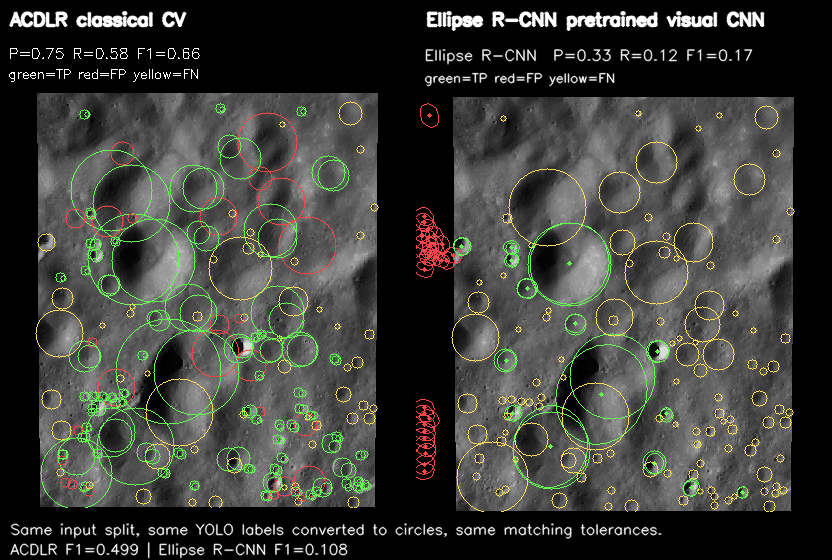
\includegraphics[width=0.92\linewidth]{figure2_acdlr_vs_ellipse_rcnn.png}
    \caption{Figura 2: visualizacao oficial da comparacao entre ACDLR e Ellipse R-CNN. O painel esquerdo mostra o metodo classico; o painel direito mostra o baseline neural pre-treinado. O rodape apresenta o $F_1$ agregado do experimento com 25 imagens.}
    \label{fig:visual-comparison}
\end{figure}

\begin{figure}[H]
    \centering
    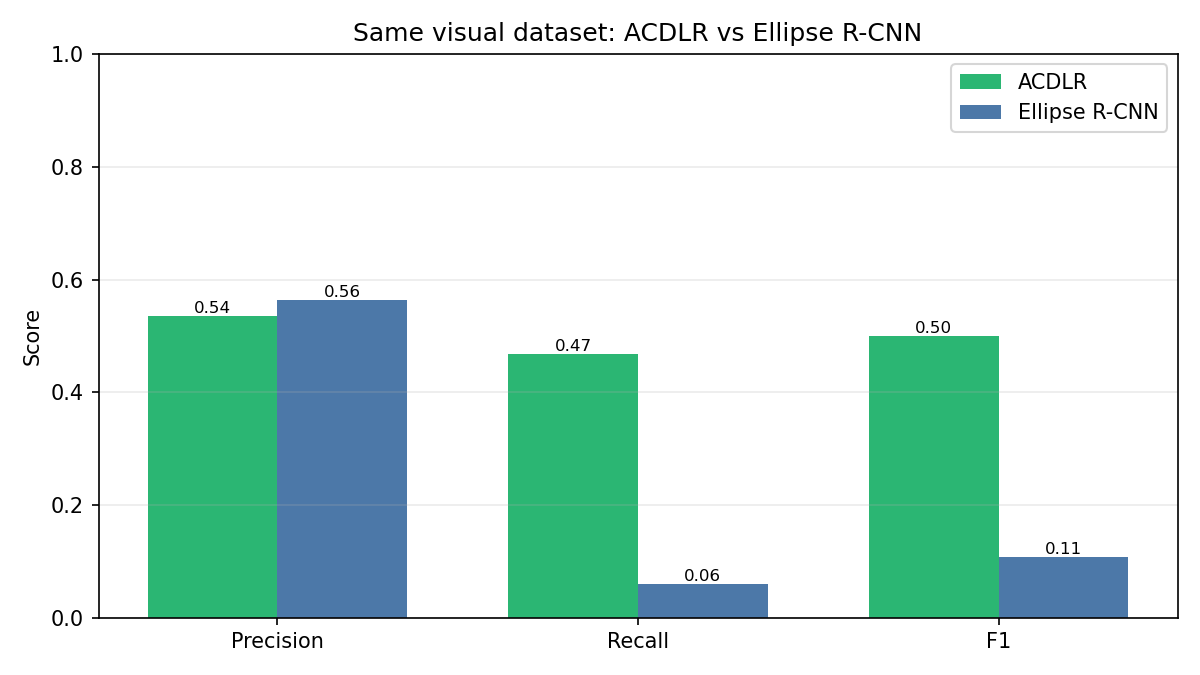
\includegraphics[width=0.78\linewidth]{figure3_metrics_chart.png}
    \caption{Figura 3: grafico oficial de precision, recall e $F_1$ no experimento com 25 imagens.}
    \label{fig:metrics-chart}
\end{figure}

\section{Estudo Qualitativo Em Outros Datasets}

Embora o foco cientifico do ACDLR seja a deteccao de crateras lunares, a estrutura do algoritmo permite estudar outros objetos circulares com contraste forte em relacao ao fundo. Essa extensao e tratada como estudo qualitativo, nao como resultado principal do artigo.

Na interface Streamlit, esses testes ficam em uma aba separada. Imagens comuns nao recebem escala fisica em metros ou quilometros. Elas sao tratadas em pixels e podem ser normalizadas para uma resolucao de entrada, por exemplo $416 \times 416$ pixels. Essa normalizacao evita comparar imagens de celular, microscopia ou rua como se tivessem escala lunar.

\subsection{Condicoes em que o algoritmo tende a funcionar}

O ACDLR tende a apresentar bons resultados fora do dominio lunar quando os objetos possuem:

\begin{itemize}
    \item contorno aproximadamente circular;
    \item contraste forte entre interior e fundo;
    \item borda relativamente continua;
    \item pouca sobreposicao entre objetos;
    \item baixa textura de fundo;
    \item escala semelhante ao intervalo de raios configurado.
\end{itemize}

Por outro lado, tende a falhar quando ha sombras alongadas, ruido visual intenso, objetos incompletos, perspectiva forte, baixa circularidade ou fundo altamente texturizado.

\subsection{Exemplo: dataset de celulas}

O dataset de celulas apresentou bons resultados qualitativos porque muitas celulas possuem formato aproximadamente circular, interior mais escuro e contraste forte em relacao ao fundo claro. Embora celulas nao sejam crateras, a geometria visual do problema se aproxima da deteccao de regioes circulares com aro ou limite visivel.

A Figura~\ref{fig:cells-study} mostra um exemplo em que o \textit{edge hint} destaca contornos de alta qualidade, e a deteccao final encontra muitos objetos circulares. Alguns erros ainda aparecem: em objetos sobrepostos, o detector pode aceitar circulos internos pequenos; em celulas deformadas, pode ajustar um circulo que nao cobre toda a estrutura. Isso ocorre porque o score do ACDLR foi desenhado para crateras, nao para segmentacao celular.

\begin{figure}[H]
    \centering
    \begin{subfigure}{0.48\linewidth}
        \centering
        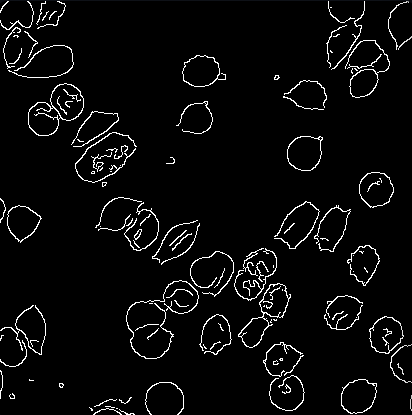
\includegraphics[width=\linewidth]{cell_edge_hint.png}
        \caption{\textit{Edge hint}.}
    \end{subfigure}
    \hfill
    \begin{subfigure}{0.48\linewidth}
        \centering
        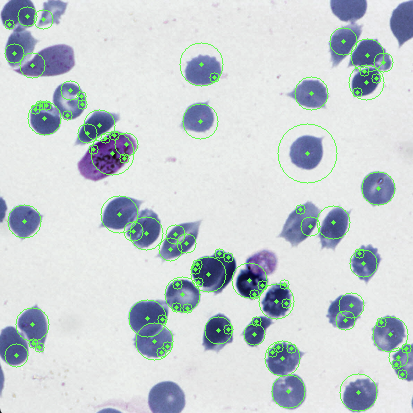
\includegraphics[width=\linewidth]{cell_detection_result.png}
        \caption{Deteccoes ACDLR.}
    \end{subfigure}
    \caption{Exemplo qualitativo em imagens celulares. O bom contraste entre celulas e fundo favorece o detector, embora o dominio nao seja lunar.}
    \label{fig:cells-study}
\end{figure}

Matematicamente, o bom desempenho pode ser interpretado pelo aumento simultaneo de $S_{\text{edge}}$, $A_{\text{cov}}$ e contraste local. Como o fundo e relativamente uniforme, regioes circulares escuras geram resposta forte no filtro multi-escala e passam nos criterios de suporte angular.

\subsection{Exemplo: buracos em ruas}

O dataset de buracos em ruas e mais dificil. Apesar de buracos tambem serem depressoes, as imagens de rua apresentam variacoes que violam pressupostos do ACDLR:

\begin{itemize}
    \item buracos raramente sao circulos regulares;
    \item a perspectiva da camera de celular distorce a geometria;
    \item asfalto possui textura, rachaduras, marcas e sujeira;
    \item sombras externas podem parecer bordas;
    \item ha grande variacao de escala entre imagens;
    \item o fundo nao e uniforme.
\end{itemize}

Nesse dominio, a borda visual pode ate aparecer forte, mas o objeto nao apresenta cobertura angular circular consistente. A funcao de score, criada para crateras, tende a rejeitar buracos muito irregulares ou aceitar regioes parciais quando a textura do asfalto cria falsos aros.

\begin{figure}[H]
    \centering
    \begin{subfigure}{0.48\linewidth}
        \centering
        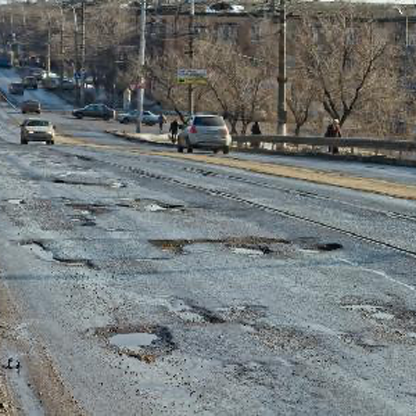
\includegraphics[width=\linewidth]{pothole_original.png}
        \caption{Imagem de rua.}
    \end{subfigure}
    \hfill
    \begin{subfigure}{0.48\linewidth}
        \centering
        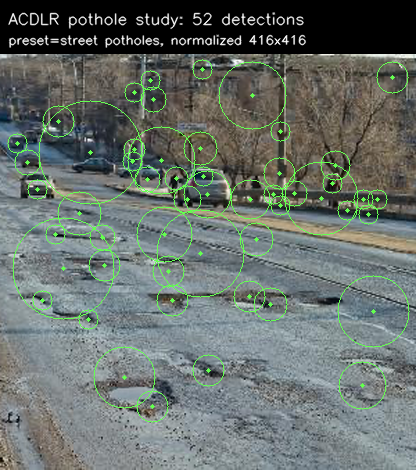
\includegraphics[width=\linewidth]{pothole_detection_result.png}
        \caption{Deteccao ACDLR.}
    \end{subfigure}
    \caption{Estudo qualitativo em buracos de ruas. O desempenho e mais instavel devido a baixa circularidade, perspectiva e poluicao visual do asfalto.}
    \label{fig:pothole-study}
\end{figure}

\subsection{Interpretacao dos testes fora do dominio lunar}

Os testes fora do dominio lunar nao devem ser apresentados como avaliacao final do ACDLR, mas como estudo de comportamento. Eles mostram que o metodo detecta bem estruturas circulares contrastantes quando os pressupostos geometricos sao satisfeitos. O caso das celulas e favoravel porque ha objetos arredondados sobre fundo claro. O caso dos buracos em rua e desfavoravel porque a forma e irregular e o fundo e visualmente poluido.

\section{Discussao}

O resultado oficial indica que o ACDLR consegue recuperar numero significativo de crateras usando apenas processamento classico. O desempenho superior ao Ellipse R-CNN no experimento de 25 imagens nao significa que metodos classicos superam redes neurais em geral. A interpretacao correta e que o baseline neural foi usado como modelo pre-treinado, sem fine-tuning local, enquanto o ACDLR foi configurado diretamente para o dominio visual do projeto.

Do ponto de vista matematico, as operacoes do ACDLR sao bem definidas: convolucoes, gradientes, estatisticas locais, limiares por percentil, matching geometrico e calculo padrao de precision, recall e $F_1$. Entretanto, a funcao de score e heuristica, nao probabilistica. Ela mede compatibilidade visual com uma cratera circular e nao representa uma probabilidade calibrada de existir cratera. De modo semelhante, a grade de risco e uma medida visual baseada nas crateras detectadas, nao uma certificacao fisica de pouso.

O principal ponto forte do ACDLR e a interpretabilidade. Cada etapa pode ser inspecionada: imagem original, CLAHE, bordas, candidatos, deteccoes e grade de risco. Isso facilita explicar por que o algoritmo falha em algumas imagens. A principal limitacao e que a funcao de score foi projetada manualmente; portanto, pode nao se adaptar a variacoes extremas de iluminacao, textura e morfologia.

No caso de imagens celulares, a boa resposta demonstra que o ACDLR tambem funciona como detector exploratorio de objetos circulares contrastantes. No caso de buracos em ruas, os resultados limitados reforcam que o algoritmo nao e um detector universal de objetos. Ele e adequado quando a geometria circular e o contraste radial sao fortes.

\section{Conclusao}

Este artigo apresentou o ACDLR, um pipeline classico para deteccao de crateras lunares e analise visual de risco. O metodo combina realce local, bordas, filtros circulares multi-escala, validacao fotometrica e geometrica, refinamento e deduplicacao. A avaliacao principal compara o ACDLR com Ellipse R-CNN usando o mesmo dataset visual, as mesmas anotacoes convertidas para circulos e as mesmas metricas.

Os resultados mostram que o ACDLR obteve maior $F_1$ no experimento oficial, principalmente por maior recall. A area experimental em outros datasets indica que o algoritmo pode identificar objetos circulares com forte contraste, como celulas, mas apresenta limitacoes em dominios com baixa circularidade e fundo poluido, como buracos em ruas.

Trabalhos futuros incluem avaliar o split de validacao completo, congelar parametros antes da avaliacao final, adicionar analise estatistica por tamanho de cratera, comparar com uma CNN fine-tunada no mesmo dataset e expandir o estudo qualitativo de generalizacao para outros objetos circulares.

\section*{Como Reproduzir}

Preparar ambiente e baseline neural:

\begin{verbatim}
python -m pip install -r requirements.txt
python scripts/setup_ellipse_rcnn_pretrained.py
\end{verbatim}

Executar o app:

\begin{verbatim}
streamlit run app.py
\end{verbatim}

Executar comparacao oficial pequena:

\begin{verbatim}
python scripts/run_acdlr_vs_ellipse_rcnn_comparison.py --max-images 25 --visual-count 8
\end{verbatim}

Os principais artefatos sao:

\begin{verbatim}
artifacts/acdlr_vs_ellipse_rcnn/comparison_report.md
artifacts/acdlr_vs_ellipse_rcnn/visual_comparison.png
artifacts/acdlr_vs_ellipse_rcnn/charts/acdlr_vs_ellipse_rcnn_metrics.png
\end{verbatim}

\begin{thebibliography}{99}

\bibitem{canny1986}
J. Canny.
\newblock A computational approach to edge detection.
\newblock \textit{IEEE Transactions on Pattern Analysis and Machine Intelligence}, 8(6):679--698, 1986.

\bibitem{pizer1987}
S. M. Pizer, E. P. Amburn, J. D. Austin, R. Cromartie, A. Geselowitz, T. Greer, B. ter Haar Romeny, J. B. Zimmerman, and K. Zuiderveld.
\newblock Adaptive histogram equalization and its variations.
\newblock \textit{Computer Vision, Graphics, and Image Processing}, 39(3):355--368, 1987.

\bibitem{hough1962}
P. V. C. Hough.
\newblock Method and means for recognizing complex patterns.
\newblock U.S. Patent 3,069,654, 1962.

\bibitem{ren2015}
S. Ren, K. He, R. Girshick, and J. Sun.
\newblock Faster R-CNN: Towards real-time object detection with region proposal networks.
\newblock \textit{Advances in Neural Information Processing Systems}, 2015.

\bibitem{ellipse2020}
W. Doppenberg.
\newblock Ellipse R-CNN: Learning to infer elliptical object from clustering and occlusion.
\newblock arXiv:2001.11584, 2020.
\newblock \url{https://arxiv.org/abs/2001.11584}

\bibitem{ellipsegithub}
W. Doppenberg.
\newblock Ellipse R-CNN repository.
\newblock \url{https://github.com/wdoppenberg/ellipse-rcnn}

\bibitem{craterdetectiongithub}
W. Doppenberg.
\newblock Crater Detection repository.
\newblock \url{https://github.com/wdoppenberg/crater-detection}

\bibitem{craterrcnn}
W. Doppenberg.
\newblock \texttt{wdoppenberg/crater-rcnn} pretrained crater model.
\newblock \url{https://huggingface.co/wdoppenberg/crater-rcnn}

\end{thebibliography}

\end{document}
